% Schematic Perron rectangle. Zeros are placed by hand, not at true ordinates.
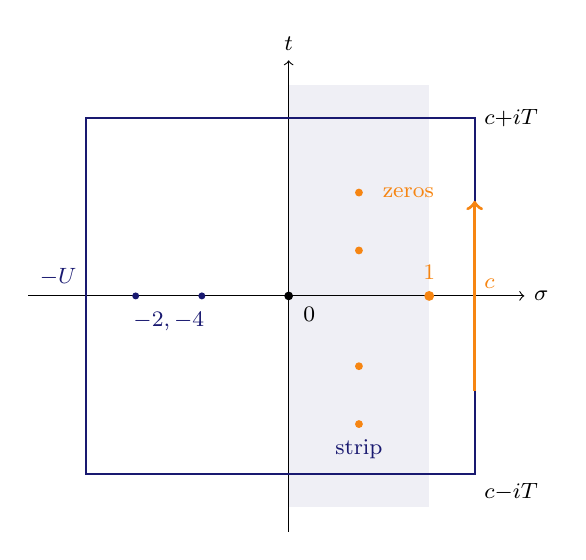
\begin{tikzpicture}[scale=1.05,every node/.style={font=\footnotesize}]
  \fill[MidnightBlue!7] (0,-2.55) rectangle (1.7,2.55);
  \draw[->] (-3.15,0)--(2.85,0) node[right] {$\sigma$};
  \draw[->] (0,-2.85)--(0,2.85) node[above] {$t$};
  \draw[MidnightBlue,thick] (2.25,2.15)--(-2.45,2.15)--(-2.45,-2.15)--(2.25,-2.15)--cycle;
  \draw[BurntOrange,very thick,->] (2.25,-1.15)--(2.25,1.15);
  \node[BurntOrange,right] at (2.25,0.15) {$c$};
  \node[MidnightBlue,above left] at (-2.45,0) {$-U$};
  \node[right] at (2.25,2.15) {$c{+}iT$};
  \node[below right] at (2.25,-2.15) {$c{-}iT$};
  \fill[BurntOrange] (1.7,0) circle (1.7pt);
  \node[BurntOrange,above] at (1.7,0.08) {$1$};
  \fill (0,0) circle (1.5pt);
  \node[below right] at (0.06,-0.02) {$0$};
  \foreach \y in {0.55,1.25,-0.85,-1.55} {
    \fill[BurntOrange] (0.85,\y) circle (1.35pt);
  }
  \node[BurntOrange,anchor=west] at (1.02,1.25) {zeros};
  \fill[MidnightBlue] (-1.05,0) circle (1.2pt);
  \fill[MidnightBlue] (-1.85,0) circle (1.2pt);
  \node[MidnightBlue,below] at (-1.45,-0.08) {$-2,-4$};
  \node[MidnightBlue] at (0.85,-1.85) {strip};
\end{tikzpicture}
